%%%%%%%%%%%%%%%%%%%%%%%%%%%%%%%%%%%%%%%%%%%%%%%%%%%%%%%%%%%%%%%%%%%%%%%%%%%%%%%
%
% Space Rover Document
%
%%%%%%%%%%%%%%%%%%%%%%%%%%%%%%%%%%%%%%%%%%%%%%%%%%%%%%%%%%%%%%%%%%%%%%%%%%%%%%%



\newcommand{\st}{Official Documentation - WP400\\
                 SIERRA BEEGND \\
                 Project SatCom 2021}       % Kurzform des Titels
\newcommand{\nr}{SatCom-21-Doc-WP400}       % Dokumentennummer
\newcommand{\ver}{0.1}                      % Version
\newcommand{\dat}{\today}                   % Datum



\input{"../texdata/format_en"}
\DeclareOldFontCommand{\sl}{\normalfont\slshape}{\@nomath\sl}
\graphicspath{{../img/}{../texdata/}}    %% Suchpfad f�r Abbildungen
\usepackage{tocloft}
\usepackage{hyperref}
\newcommand{\mailto}[1]{\href{mailto:#1}{#1}}
\renewcommand\cftchapnumwidth{2.8em}
\begin{document}
\renewcommand{\thisauthor}{SatCom 2021}
%%%%%%%%%%%%%%%%%%%%%%%%%%%%%%%%%%%%%%%%%%%%%%%%%%%%%%%%%%%%%%%%%%%%%%%%%%%%%%%
%
% Titelseiten
%
%%%%%%%%%%%%%%%%%%%%%%%%%%%%%%%%%%%%%%%%%%%%%%%%%%%%%%%%%%%%%%%%%%%%%%%%%%%%%%%


\belowpdfbookmark{Title}{titlepage}

\begin{titlepage}
  \begin{tikzpicture}[
  remember picture,
  overlay
  ]
  \node [anchor = north west] at ([xshift = +10mm, yshift = -10mm]current page.north west) {
    
\includegraphics[height = 20mm]{tuBerlinLogoSchwarz.pdf}
  };
  \end{tikzpicture}
  \begin{tikzpicture}[
  remember picture,
  overlay
  ]
  \node [anchor = north ] at ([xshift = +7 mm, yshift = -10mm]current page.north) {
    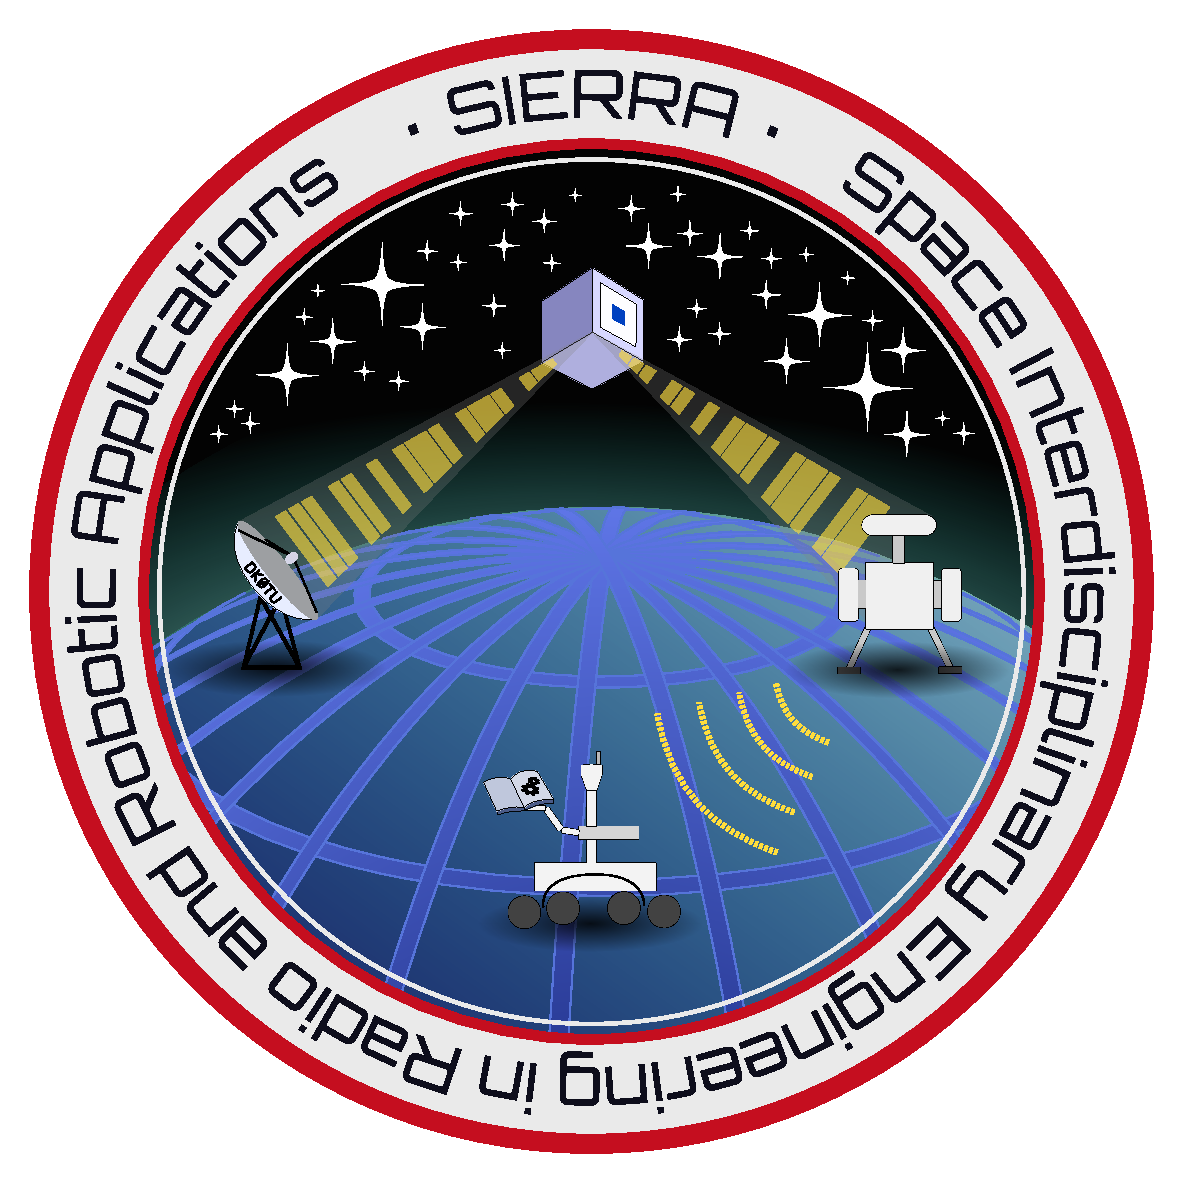
\includegraphics[height = 90mm]{sierra_r4.pdf}
  };
  \end{tikzpicture}
  \begin{center}
    \hspace{0pt}\vfill

    %\large Space Interdisciplinary Engineering in Radio and Robotic Applications \\ \hspace{0pt}

    \huge\textbf{Official Documentation} \\ \vspace{20pt}

    \large{Berlin Experimental and Educational Ground Station}

    \vfill

    \normalfont\normalsize Document: \nr \\
    Version: \ver\\
    Date: \dat

    \vfill

    %
\includegraphics[height=\hh]{../../global_references/tuBerlinLogoRot}
    %
\includegraphics[height=\hh]{../../global_references/tuBerlinLogoSchwarz}

    \normalfont\normalsize \hspace{0pt}\\
    Technische Universit\"at Berlin\\
    Department of Aeronautics and Astronautics\\
    Chair of Space Technology\\
    Office F 6\\
    Marchstra�e 12--14\\
    10587 Berlin

    Tel.: 030 / 314-21305\\
    Fax: 030 / 314-21306
  \end{center}
\end{titlepage}


%%%%%%%%%%%%%%%%%%%%%%%%%%%%%%%%%%%%%%%%%%%%%%%%%%%%%%%%%%%%%%%%%%%%%%%%%%%%%%%

\begin{titlepage}
  \begin{center}
    \textbf{\huge{Technical Note}\\\hspace{0pt}}
    %\textbf{\large{This is an mple headline}\\\hspace{0pt}}
    
    \ \\
    \ \\
    \textbf{Version History\\\hspace{0pt}}
    
    \begin{tabular*}{\textwidth}
      {%
        @{}p{0.1\textwidth}
        p{0.15\textwidth}
        p{0.35\textwidth}
        p{0.3\textwidth}@{}
      }
      \toprule
      Version & Date & Changes & Processor \\
      \midrule
      0.1 & 2021-07-05 & Document creation  & Alexis Cabana-Loriaux \\
      \bottomrule
    \end{tabular*}%
    
    \vfill
    
    \thispagestyle{TUB}
    
    \pagebreak
    
     
    
    
    
    
  \vfill

     \end{center}%
  \thispagestyle{TUB}%
\end{titlepage}

%%%%%%%%%%%%%%%%%%%%%%%%%%%%%%%%%%%%%%%%%%%%%%%%%%%%%%%%%%%%%%%%%%%%%%%%%%%%%%%


\clearpage

%%%% INHALT %%%%
\pagenumbering{Roman}
\addcontentsline{toc}{chapter}{Table of Contents}
\tableofcontents


\subpdfbookmark{Contents}{tables}
\belowpdfbookmark{Contents}{toc}

\clearpage
\def\thechapter{\arabic{chapter}00}
\setcounter{chapter}{3}
\chapter{Portable Rotator Concept}
\pagenumbering{arabic}

%%%%%%%%%%%%%%%%%%%%%%%%%%%%%%%%%%%%
% your documentation here
%%%%%%%%%%%%%%%%%%%%%%%%%%%%%%%%%%%%

\end{document}
